\documentclass{article}

\usepackage[utf8]{inputenc}
\usepackage[T1]{fontenc}
\usepackage{lipsum}
\usepackage{graphicx}
\usepackage{amsmath}
\usepackage[margin=1in]{geometry}
\usepackage{titlesec}
\usepackage{enumitem}

\titleformat{\section}
{\LARGE\bfseries}{\thesection}{1em}{}

\titleformat{\subsection}
{\Large\bfseries}{\thesection}{1em}{}

\begin{document}

\pagestyle{empty}

\section*{Diagramma dei casi d'uso}
\large
\subsection*{Introduzione}
Obiettivi:
\begin{enumerate}
    \renewcommand{\labelenumi}{-}
    \itemsep0em
    \item Identificare i \textit{casi d'uso}
    \item Connettere i casi d'uso rispetto agli obiettivi dell'\textit{attore principale}
    \item Mantenere uno stile \textit{essenziale}, non troppo informativo, poichè potrebbe rendere maggiormente difficile l'individuazione del \textit{goal}
    \item Adottare uno \textit{sviluppo iterativo} 
\end{enumerate}
\textbf{Use case} spesso è indicato come il meccanismo per scoprire e registrare i requisiti, di carattere \textit{funzionale}. La scrittura dei \textit{casi d'uso} è un eccellente tecnica per capire e descrivere ciò che il \textit{sistema} debba implementare, rispetto ad una totalità di influenze esterne che creino la situazione ideale per poter proseguire con il compimento dell'obiettivo principale da parte del \textit{soggetto}.
\textbf{UP}, ossia \textit{Unified Process}, indica un certo modello dei casi d'uso, definito come \textbf{modello comportamentale}, per cui fortemente connesso rispetto ai \textit{comportamenti} degli elementi trattati.\vspace*{14pt}\\
I \textit{diagrammi} dei \textit{casi d'uso} sono \textbf{diagrammi comportamentali} utilizzati per descrivere un insieme di azioni, o meglio \textit{behavior}, che un sistema deve svolgere insieme ad uno o più utenti esterni al sistema. Inoltre, carattere imprescindibile di tale modellazione, prevede che ogni \textit{use case} fornisca un \textbf{risultato di valore}, per gli utenti con cui interagiscono oppure per gli \textit{stakeholders}. \textit{Customers} e \textit{final users} pongono certi obiettivi, detti \textit{needs}, i quali richiedono che \textit{sistemi} siano in grado di rendere chiaro il loro \textbf{connubio}.\vspace*{14pt}\\
Differenti sono gli approcci dettati, tuttavia le strategie migliori riguardano un uso semplice e famigliare degli strumenti messi a disposizione, poichè rendono più semplice la lettura del modello, contribuiscono alla ricerca dei requisiti necessari e abbassa il rischio di perdere l'obiettivo su cui fonda l'intera architettura, definito anche \textit{missing the mark}.\\
Infatti il primo step ricade nella comprensione del problema assieme all'individuazione dei requisiti funzionali che comporranno i casi d'uso, affinchè siano comprensibili da parte dei portatori di interesse. Tuttavia, quest'ultimo passaggio rappresenta la maggiore difficoltà di questo modello, ossia la decisione e scoperta di cosa sia potenzialmente necessario; durante una prima fase di analisi potrebbero essere inseriti dei \textit{layer sofistaticati-aggiuntivi}, i quali solitamente oscurano il reale proseguimento del \textit{mark}.\vspace*{14pt}\\
Per cui, ricapitolando, il diagramma dei casi d'uso è utilizzato per specificare:
\begin{enumerate}
    \renewcommand{\labelenumi}{-}
    \itemsep0em
    \item I requisiti esterni degli stakeholders, funzionali rispetto a quanto il sistema debba implementare
    \item Le funzionalità offerte dal sistema per tutti i final user esterni
    \item Rispettare i limiti secondo cui il sistema debba sottostare, defininendo come tale ambiente debba interagire con il soggetto pur di proseguire verso il \textit{path} voluto
\end{enumerate}

\subsection*{Elementi del diagramma}
In questa sezione si analizzano gli elementi comuni ad un qualsiasi diagramma dei casi d'uso, descrivendo successivamente caratteristiche uniche rispetto alle strategie elencate.\vspace*{14pt}\\
\textit{Definizione informale}\\
Un \textbf{attore} è qualcosa caratterizzato da un comportamento, come una persona, un computer system oppure un'organizzazione.\vspace*{14pt}\\
Per cui, descrivendone maggiormente il ruolo svolto, un \textbf{attore} è un \textbf{classificatore comportamentale}, ossia un'entità che interagisce con il sistema implementato o ideato mediante \textbf{interazioni}, quali, semplicemente, l'invio di segnali o di dati.\vspace*{14pt}\\
\textit{Definzione informale}\\
Uno \textbf{scenario}, definito anche \textit{istanza} del caso d'uso, indica un preciso percorso attraversando certi e specifici \textit{use case}.\vspace*{14pt}\\
Quindi il modello comportamentale trattato è definito mediante un insieme di scenari fallimentari o di successo, in relazione al conseguimento dell'obiettivo dell'attore principale, adeguandosi ai comportamenti illustrati all'interno dei singoli casi d'uso. E' bene sottolineare come ogni caso d'uso rappresenti uno specifico requisito funzionale, posto al di fuori del diagramma, dove solamente mediante interazioni è possibile stabilire un path per cui il sistema sia in grado di raggiungere l'obiettivo.\\
Sono definiti differenti formati del diagramma dei casi d'uso, legati ad una descrizione maggiormente esaustiva oppure funzionale; si ribadisce quale sia comunque il caposaldo su cui regge tale modello comportamentale, mantenere il \textit{focus} sull'obiettivo principale, evitando di offuscare la mente tramite la lettura di aspetti non del tutto incidenti e pertinenti per la reale comprensione e analisi del diagramma.\vspace*{14pt}\\
\textit{Esempio}\vspace*{2pt}\\
Si osserva ora una rappresentazione grafica.\\ Alla sinistra è posta un esempio meno dettagliato, mentre corrispettivamente è posto un livello informativo più complesso.\vspace*{14pt}
\begin{center}
    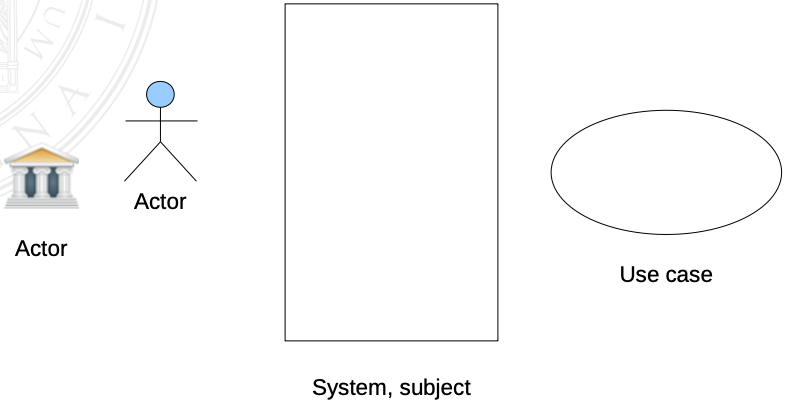
\includegraphics[width=0.8\textwidth]{foto 1.png}
\end{center}
\pagebreak
Non esiste un formato migliore, tuttavia la \textit{key thing} consiste nella descrizione di dettagli dello scenario di successo e delle sue estensioni, in relazione anche a casi fallimentari,  ossia quei determinati \textit{path} che non competono per il conseguimento del \textit{mark}, rappresentando comunque sia un \textit{end point}.\\
Spesso la domanda da porsi per un qualsiasi modello adottato, consiste in cosa dovrebbe essere riportato all'interno dei differenti casi d'uso. La risposta, anche se scontata, prevede di riportare tutto ciò che permetta di soddisfare i portatori di interesse, evitando di adottare un livello specificativo troppo elevato, poichè potrebbe risultare essere fuorviante.

\subsection*{Modello di casi d'uso e diagramma dei casi d'uso}
\large
Un diagramma UML per un caso d'uso \textbf{NON} è un modello di caso d'uso! Il diagramma può essere visto come un \textbf{sommario}, non avendo al suo interno aspetti fondamentali come i dettagli sulle fasi di interazione e quando il caso d'uso viene applicato, le condizioni pre/post, ecc. Inoltre, \textbf{non esiste} una notazione standard per rappresentare un modello di caso d'uso, ma esistono molti \textbf{template} utilizzati in base al caso specifico. I template possono essere \textbf{molto dettagliati o più semplici}, in base ai differenti casi e dal team di sviluppo (è fondamentale rimanere costanti). In ogni template sono presenti diverse \textbf{sequenze}, che ci indicano i diversi casi possibili durante una ipotetica esecuzione. Spesso, oltre alla sequenza che illustra l'esecuzione ottimale (\textit{Happy path}), vengono indicate sequenze alternative che portano comunque all'obiettivo finale seguendo un percorso diverso. Può anche esserci una sequenza (\textit{Exceptions}) dove non viene raggiunto l'obiettivo.

\subsection*{Diagramma dei casi d'uso}
\large
UML mette a disposizione il \textit{diagramma dei casi d'uso}, illustrando i differenti \textit{attori}, \textit{use case} e \textit{relazioni} che intercorrono. Le entità principali possono essere riportate come segue.\vspace*{14pt}\\
\textit{Attore}\\Il quale ricalca la stessa descrizione informale data precedentemente, ossia rappresenta un certo \textbf{classificatore comportamentale}.\vspace*{14pt}\\
\textit{Soggetto}\\Il \textbf{soggetto} è il sistema sotto analisi, al quale vengono applicati i diversi casi d'uso. Il soggetto può essere una qualsiasi entità, ossia un sistema software, sistema fisico oppure un sottosistema del soggetto. Il soggetto è un \textbf{classificatore di casi d'uso} che ha il ruolo di \textit{soggetto}.\vspace*{14pt}\\
\textit{Casi d'uso}\\Un \textbf{caso d'uso} è anch'esso un \textit{classificatore comportamentale} che indica quali comportamenti possano essere descritti conseguendo in una \textbf{sequenza di azioni}, pur sempre eseguite dal sistema per ottenere un  risultato \textbf{osservabile}, sperando che appartenga alla zona di interesse degli stakeholder.\vspace*{14pt}\\
\begin{center}
    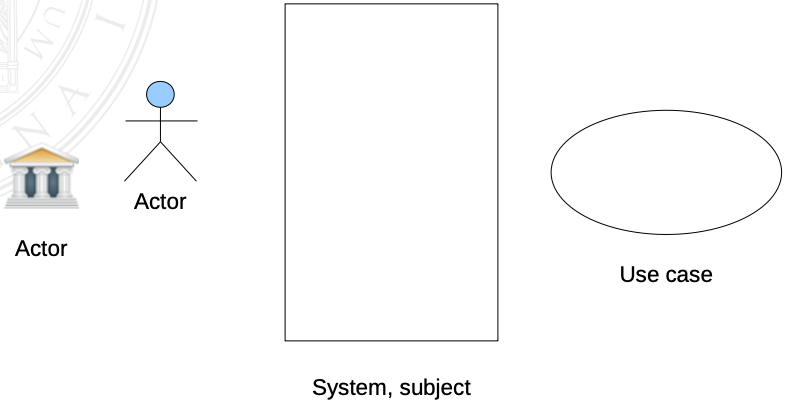
\includegraphics[width=0.6\textwidth]{foto 2.png}
\end{center}

\subsection*{Relazioni}
\large
In un diagramma simile le interazioni sono espresse mediante relazioni, le quali sono di vario genere, implementate a seconda del contesto.\vspace*{14pt}\\
\textbf{Relazioni attori}\vspace*{14pt}\\
\textit{Generalizzazione}\\La \textbf{generalizzazione} tra attori è rappresentata graficamente come una linea direzionata. Adottata per esprimere l'ereditarietà, per cui da un certo attore padre posso rescindere un infinito numero di attori discendenti.\vspace*{14pt}\\
\textit{Associazione tra attori e casi d'uso}\\Ogni caso d'uso specifica delle funzionalità utili che il soggetto fornisce agli attori. Queste funzionalità devono essere inizializzate da un attore. L'associazione posta tra un attore e un caso d'uso può essere solo \textbf{binaria}.\vspace*{14pt}\\
\textbf{Relazioni casi d'uso}\vspace*{14pt}\\
\textit{Generalizzazione}\\Come avviene per gli attori la \textbf{generalizzazione} tra casi d'uso avviene tramite un freccia direzionata, dove la stessa freccia è posta dal caso \textit{specifico} a quello \textit{generico}.
\begin{center}
    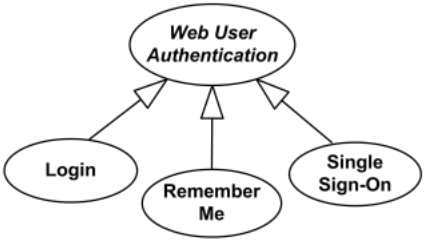
\includegraphics[width=0.4\textwidth]{foto 3.png}
\end{center}
\textit{Extend}\\L'\textbf{extend} è una relazione che indica come e quando il comportamento definito in maniera \textit{opzionale}, il quale estende il caso d'uso in questione, possa devenire parte del comportamento attivo. Le relazioni di questo genere vengono rappresentate graficamente come una freccia tratteggiata avente una punta aperta, posta dal caso esteso verso il caso base; al di sopra è posta la denominazione \textbf{<<extend>>}.
\begin{center}
    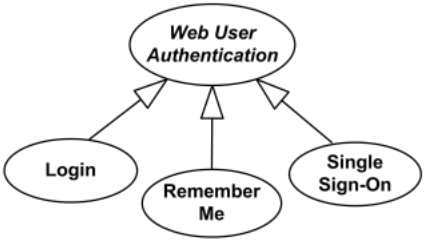
\includegraphics[width=0.4\textwidth]{foto 4.png}
\end{center}
come da rappresentazione grafica si evidenzia la presenza di un'etichetta, definita \textbf{punto di estensione}. Un punto di estensione è attuato qualora un caso d'uso specifico abbia un comportamento opzionale, ossia un'estensione rispetto al proprio \textit{behavior standard}. Ogni punto di estensione deve avere un nome, unico e univoco nella modellazione del diagramma.\vspace*{14pt}\\
\textit{Include}\\Una relazione di \textbf{inclusione} è una relazione diretta tra due o più casi d'uso, adoperata quando un comportamento richiesto, quindi relativo al passaggio da requisito funzionale a behavior, non è opzionale, in cui lo stesso use case di base ne è strettamente dipendente. Essa è rappresentata mediante una freccia tratteggiata con una punta aperta, dove la direzione segue dal caso d'uso specifico verso quello base; inoltre viene posta al di sopra la denominazione \textbf{<<include>>}.
\begin{center}
    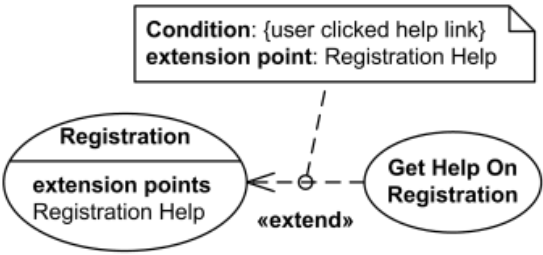
\includegraphics[width=0.4\textwidth]{foto 5.png}
\end{center}

\subsection*{Main sequence}
\large
Come già detto, il diagramma dei casi d'uso non rappresenta l'unico metodo di analisi e descrizione, in relazione allo studio di modelli comportamentali, sono presenti anche approcci molto più informativi, i quali hanno un obiettivo contrario rispetto a quanto detto prima.\vspace*{14pt}\\
Un'alternativa valida è denominata \textbf{main sequence} oppure \textbf{happy path scenario}. E' in grado di descrivere il path di successo che soddisfi gli interessi degli stakeholders. Rispetto ad un qualsiasi diagramma, questa tipologia, non permette di esprimere ogni altra condizione o ramificazione. Spesso è adottata per analizzare tre punti successivi:
\begin{enumerate}
    \renewcommand{\labelenumi}{-}
    \itemsep0em
    \item Interazioni tra gli attori 
    \item Il sistema di validazione dei comportamenti consentiti dal sistema
    \item Il cambiamento di stato del sistema, poichè soggetto ad influenze esterne 
\end{enumerate}
Tuttavia, spesso è dedicata una sezione apposita alle \textbf{estensioni}, o meglio definite \textbf{extensions}. Sono descritti gli scenari, sia di successo che fallimentari, i quali potrebbero risultare più complessi rispetto al main sequence. Gli \textit{alternative flows} sono suddivisi in due entità di equivalente importanza, le condizioni e le azioni.\vspace*{14pt}\\
\textit{Esempio}\vspace*{2pt}\\
\textit{MAIN SUCCESS SEQUENCE (a.k.a. Happy path)}:
\begin{enumerate}
    \itemsep0em
    \renewcommand{\leftmargin}{1cm}
    \item L'utente seleziona l'opzione per entrare in un nuovo trasferimento
    \item Il sistema mostra il modulo per effettuare il trasferimento (conto destinatario, dettagli, importo, data)
    \item L'utente inserisce i dati nel modulo ed effettua l'ordine
    \item Il sistema mostra il messaggio di accettazione dell'ordine
\end{enumerate}
\textit{EXTENSIONS}:
\begin{enumerate}[label={\arabic*}, leftmargin=1cm]
    \item[3a] Importo non disponbile:
\end{enumerate}
\begin{enumerate}[label={\arabic*}, leftmargin=1.7cm]
    \item[3a.1] Il sistema mostra un messaggio di errore e torna allo step 2
\end{enumerate}

\subsection*{Metodo di uso}
\large
I casi d'uso sono definiti per soddisfare gli obiettivi degli utenti, che interagiscono con il sistema, e soprattutto dell'attore principale. Una basica procedura può essere:
\begin{enumerate}
    \renewcommand{\labelenumi}{-}
    \itemsep0em
    \item Scegliere il sistema circondario, in relazione a quale ambiente debba essere sviluppato e modellato
    \item Identificare l'attore principale, solitamente posto alla sinistra, il quale compie tutte le azioni necessarie pur di conseguire nell'obiettivo voluto
    \item Per ogni attore identificare i loro obiettivi
    \item Definire i casi d'uso che consentono di soddisfare i differenti requisiti funzionali
\end{enumerate}

\subsection*{HomeWork}
\large
Un \textit{blog} è una \textit{web application} che contiene una serie di messaggi (\textit{post}) datati su diversi argomenti. I messaggi vengono postati dal creatore del blog che li mette online. L'autore può associare ad ogni messaggio una o più categorie (tramite delle parole chiave). \\
I visitatori del blog possono commentare i messaggi; i commenti, se approvati dal moderatore (di solito è il creatore del blog), appaiono in una sezione specifica sotto il messaggio originale. \\ \\
Partiamo capendo quale sia il soggetto, ovvero la nostra \textit{web application}. Procediamo poi trovando gli attori:
\begin{enumerate}
    \renewcommand{\labelenumi}{-}
    \itemsep0em
    \item Creatore del blog
    \item Visitatore
    \item Moderatore
\end{enumerate}
L'obiettivo del creatore del blog è quello di \textbf{pubblicare i messaggi}.\\
Vediamo ora un modello di casi d'uso d'esempio per questo caso:
\begin{center}
    
\includegraphics[width=0.6\textwidth]{foto 6.png}
\end{center}
Come possiamo osservare, abbiamo i nostri tre attori (creatore del blog, visitatore e moderatore) ed i loro obiettivi.
Un'altra possibile soluzione poteva essere la seguente:
\begin{center}
    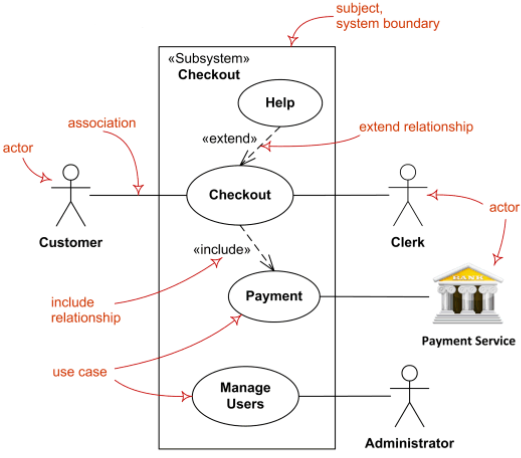
\includegraphics[width=0.6\textwidth]{foto 7.png}
\end{center}
In questo caso dovremmo specificare in qualche modo che non possono essere eseguite entrambe le operazioni (approve e reject), ma soltanto una per commento (magari tramite l'utilizzo di XOR). Tra i due approcci è preferibile il primo, non dovendo specificare l'esclusività e per un approccio meno confusionario rispetto al secondo.
Se volessimo mantenere un modello funzionale più semplice:
\begin{center}
    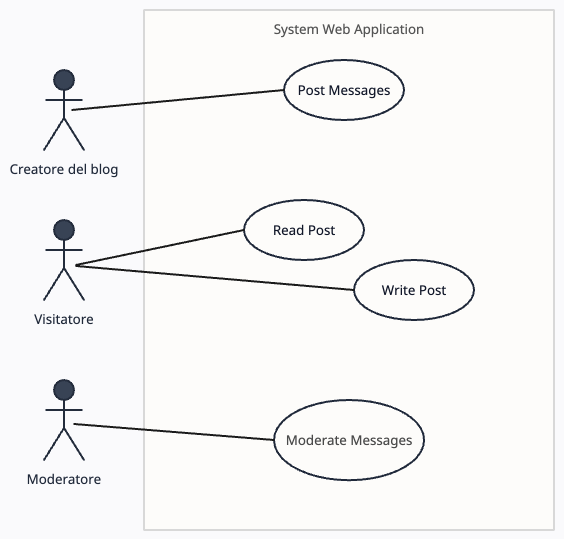
\includegraphics[width=0.6\textwidth]{foto 8.png}
\end{center}
Questa soluzione è buona, anche se meno dettagliata. In questo caso però il più completo è migliore, perchè non risulta essere troppo confusionario. Ripensando al ciclo di vita di un modello di casi d'uso, questa potrebbe essere la fase iniziale della modellazione.\\ \\
Se avessimo voluto usare un template di caso d'uso semplice, avremmo ottenuto (stiamo considerando l'obiettivo \textit{write comment}):
\begin{enumerate}
    \renewcommand{\labelenumi}{-}
    \item \textbf{UC1}: write comment
    \item \textbf{Actors}: visitor 
    \item \textbf{Pre-condition}: utente visualizza il messaggio
    \item \textbf{Main Sequence}:  
    \begin{enumerate}
        \item utente scrive il commento
        \item utente invia il commento
        \item sistema conferma la ricezione del commento
    \end{enumerate}
    \item \textbf{Alternative Sequence}: il messaggio contiene linguaggio non appropriato\\
    (c1) Il sistema cancella il commento
    \item \textbf{Post-condition}: il messaggio viene aggiunto alla lista dei messaggi da moderare
\end{enumerate}
\end{document}